\documentclass[12pt]{article}
\usepackage[utf8]{inputenc}
\usepackage[T2A]{fontenc}
\usepackage[mongolian]{babel}
\usepackage{graphicx}
\usepackage{amsmath}
\usepackage{amssymb}
\graphicspath{{zurag/}}

\begin{document}
	\section{Оршил}
   Өнөө үед мэдээллийн технологи асар хурдацтай хөгжиж байгаагаас байгууллага , аж ахуйн нэгжийн 
   үйл ажиллагаа хэв маяг ч өөрчлөгдөж байна . Үүнийг дагаад албан байгууллага хувь хүмүүс бүгд 
   компьютер буюу тооцоолон бодох машинтай салшгүй холбоотой болсон  ба тэр дундаа хүний хийх ажлыг хөнгөвчлөх,
   ажлын бүтээмжийг өндөрсгөх зэрэг асуудал нь нэн чухлаар тавигдаж байгаа. 
   Өнөөгийн мэдээллийн зуун гэж нэрлэгдсэн энэ үед хэн мэдээлэл сайн олж чадаж байна тэр чинээгээрээ амжилт олж чадах болсон.
   Иймд аливаа байгууллагын үйл ажиллагааг зохион байгуулах, мэдээллийн урсгалыг тодорхой болгож, мэдээллийг хурдан дамжуулах
   шаардлага зайлшгүй тулгар ч байна. Иймд интернет болон компьютерийн тусламжтай Сургуулийн цахим хуудсийг ажиллуулах нь
   багш оюутнууд ажил хичээлээ явуулхад тулгарсан ямар нэг асуудлийг шийдхэд нэн чухал үүрэг гүйцэтгэх юм.
   
   \subsection{Системийн зорилго}
    Их сургуулийн олон нийтийн сүлжээний Зөвлөх багшийн систем нь оюутан бүртгэх, дүнгийн мэдээлэл харах , төлөвлөгөө гаргах зэрэг нь хүндрэлтэй байдаг тул энэ үйл ажиллагаануудыг хялбарчлах зорилготой юм.
   	\section{Судалгаа}
       Энэ хөгжүүлэх гэж байгаа програм  нь Facebook-н app адилхан . Өөрийн програмын нэг модул болох 
      Зөвлөх багш (Adviser)нь оюутантай харицах , зөвөлөгөө ,зар мэдээ мэдээллийг цаг тухайд нь өгөх үүрэгтэй .
      Энэхүү модулийн хэрэглэгчид нь тухайн сургуулийн багш болон туслах багш бас оюутан юм. Оюутануудтайгаа харицахад 
      хялбар болох ба бүх оюутантай эрх тэгш харицах эрхийг олгох  болон эцэг эхтэйн холбогдоход хялбар болно . 
   
	\section{Класс диаграмм}
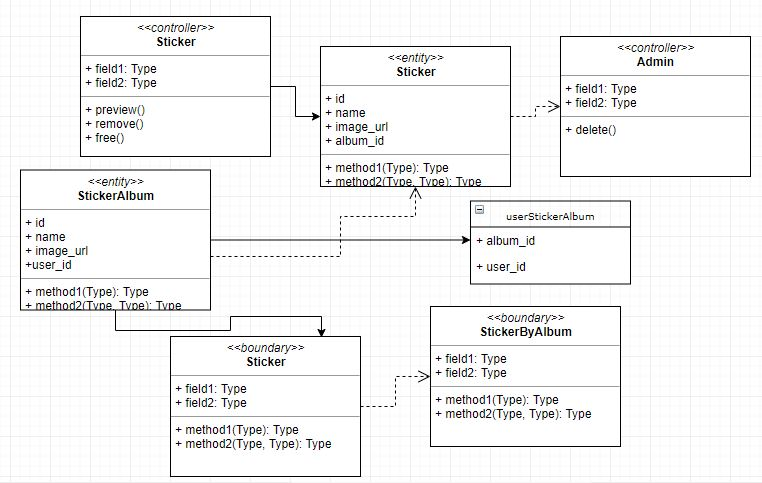
\includegraphics[scale=0.5]{class.png} 
   	
\end{document}